\documentclass[a4paper,12pt]{article}
\usepackage{times}
\usepackage[francais]{babel}
\usepackage[utf8x]{inputenc}

\usepackage[T1]{fontenc}
\usepackage{hyperref}
\usepackage[shortlabels]{enumitem}
\setlength{\parindent}{0pt}
\setlength{\parskip}{\baselineskip}

\usepackage{amsmath}
\usepackage{amssymb}

\usepackage{graphicx}
\graphicspath{ {res/} }

\usepackage{pdfpages}
\usepackage{pdflscape}

\usepackage{listings}
\usepackage{longtable}
\lstset{literate=
{é}{{\'e}}1
{è}{{\`e}}1
{ê}{{\^e}}1
{à}{{\`a}}1
{â}{{\^a}}1
}
\lstset{language=C++,
                basicstyle=\footnotesize,
                keywordstyle=\footnotesize\color{blue},
                otherkeywords={override,nullptr}
}
\definecolor{orange}{rgb}{0.8,0.4,0.0}
\definecolor{darkblue}{rgb}{0.0,0.0,0.6}
\definecolor{cyan}{rgb}{0.0,0.6,0.6}
\lstdefinelanguage{JSON}
{
  basicstyle=\normalsize,
  columns=fullflexible,
  showstringspaces=false,
  commentstyle=\color{gray}\upshape,
  morestring=[b]",
  morestring=[s]{>}{<},
  morecomment=[s]{<?}{?>},
  stringstyle=\color{orange},
  identifierstyle=\color{darkblue},
  keywordstyle=\color{blue},
  morekeywords={string,number,array,object}% list your attributes here
}

\sloppy

\setlength{\topmargin}{0cm}
\setlength{\headsep}{0.in}
\setlength{\headheight}{0.in}
\setlength{\evensidemargin}{0cm}
\setlength{\oddsidemargin}{-1cm}
\textwidth 18cm
\textheight 25cm

\begin{document}

\thispagestyle{empty}

\begin{titlepage}

\vspace*{2cm}

\begin{center}\textbf{\Huge Projet }\end{center}{\Large \par}

\begin{center}\textbf{\large Attigui Youness - Quellier Louis}\end{center}{\large \par}

\vspace{2cm}

  \begin{figure}[ht]
        \centering
        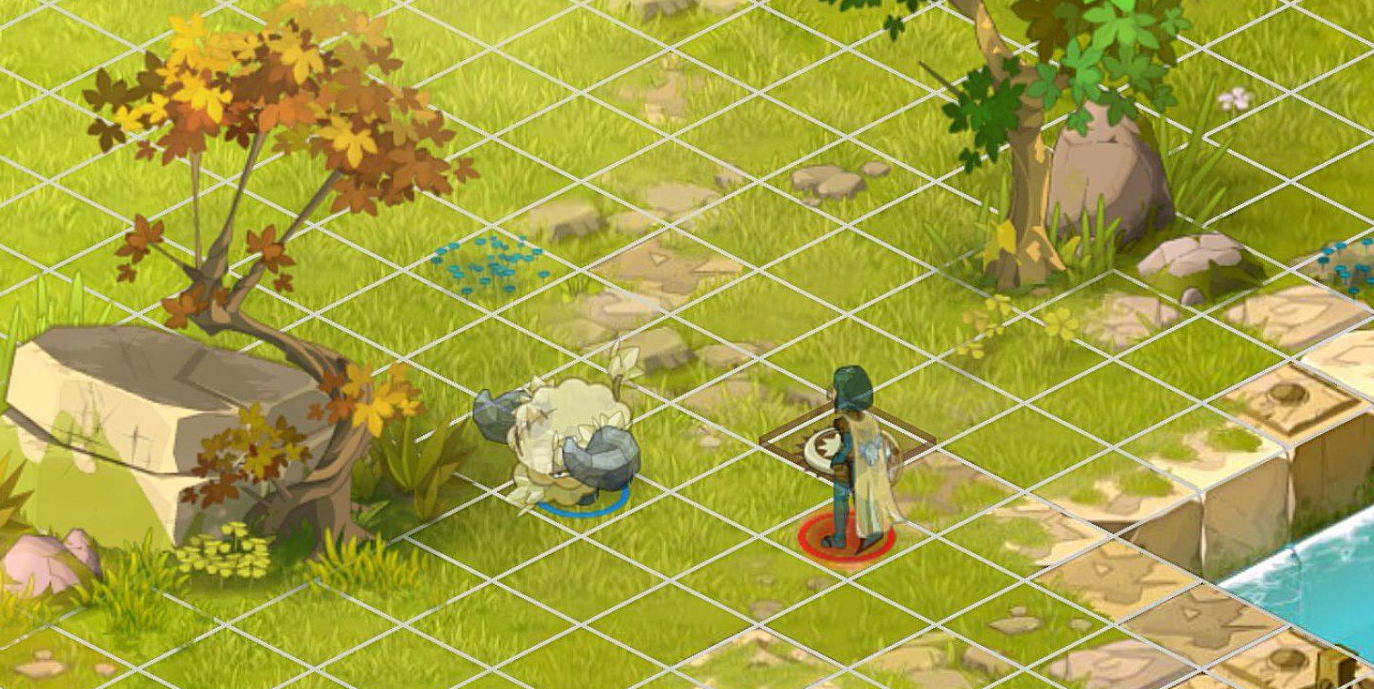
\includegraphics[width=\textwidth]{dofus.png}
        \caption{Exemple du jeu}
    \end{figure}


\clearpage

{\small
\tableofcontents
}

\end{titlepage}

\clearpage
\section {Présentation Générale}

\subsection{Archétype}
    Pour ce projet nous nous inspirons du gameplay du jeu \href{http://www.jeuxvideo.com/jeux/pc/00013232-dofus.htm}{"Dofus"}. Il s'agit d'un jeu de stratégie au tour par tour où il est possible de se déplacer de carte en carte pour combattre des ennemis et gagner de l'équipement et de l'expérience permettant d'améliorer son personnage et d'avancer plus loin dans le monde.

\subsection{Règles du jeu}
    Vous incarnez un héros auto-proclamé qui vient de fonder sa guilde d'aventurier dans le but de libérer le royaume de l'emprise du roi démon.
    
    % description aventure (début, victoire, défaite)
    L'aventure commence avec une arme basique au choix, combiné avec un élément de prédilection. Ces armes pourront être trouvées ou achetées et gagneront des niveaux selon le nombres d'ennemis vaincus, débloquant ainsi des bonus de statistiques ainsi que des nouvelles actions, pouvant également être améliorées. Ce niveau est inhérent à l'arme et sera alors conservé lors du transfert vers un autre personnage. 

	% description stats des personnages / ennemis
    Tous les personnages du jeu possèdent en plus de leur arme un ensemble de caractéristiques propres à chacun :
    \begin{itemize}[noitemsep,topsep=0pt]
        \item pv : point de vie (s'ils tombent à 0, le personnage meurt et lâche son matériel sur la case sur laquelle il se trouvait)
        \item pa : point d'action (permettent d'utiliser les actions associées aux armes)
        \item pm : point de mouvement (permettent de se déplacer)
        \item éléments : eau/terre/feu/air
    \end{itemize}

    % description map
    Les différents éléments (l'eau, la terre, le feu et l'air) font partie intégrante de ce monde et sont au coeur des stratégies de combat. Des bonus et malus de type élémentaire sont appliqués selon l'attribut du joueur, de son arme et de la case du terrain sur lequel il est placé. C'est à vous d'utiliser le terrain et vos compétences à votre avantage.
    
    % mouvement map et mission
    Au cours de l'histoire, d'autres aventuriers rejoindront votre guilde afin de vous aider dans votre tâche et vous serez engagés pour effectuer des missions variées afin de gagner de l'or pour acheter de nouvelles armes ou recruter de nouveaux mercenaires.
    
    En tant que guilde indépendante vous êtes libres de vous déplacer à votre guise dans le royaume pour accomplir les missions dans l'ordre que vous souhaitez. Néanmoins, dans ce monde il n'existe pas d'organisme régissant les missions, celles-ci vous sont confiées lorsque vous arrivez sur les lieux.
    
    Par moments vous devrez défendre une ville contre une attaque adverse, parfois vous devrez protéger un voyageur surpris par une embuscade ennemie ou souhaitant une escorte, d'autres fois vous devrez détruire une base fortifiée mais le plus souvent vous devrez simplement éliminer tous les adversaires présents dans une zone.
    
    % description terrain
    Un combat se déroule sur un des terrains de la carte du monde. Chaque terrain est composé d'un nombre fixe de cases. Chaque case est associé à un élément (eau, terre, feu, air, neutre). Le déploiement des personnages s'effectue au début du combat sur une zones prédéterminée dépendant de la direction d'arrivée, la disposition à l'intérieur de cette zone étant libre.
    
    % réputation
    Au cours de votre aventure votre guilde acquiert une certaine notoriété dans le royaume, celle-ci peut aussi bien être positive que négative, influant sur vos interactions avec les différents personnages. Au fil de vos rencontres, vous pourrez refuser certaines missions pour diverses raisons mais cela fera diminuer votre réputation. Le degré de réussite ou d'échec des missions acceptées modifiera également cette réputation.
    
    Si votre guilde a trop mauvaise réputation, vous serez exécutés en tant que criminel et l'aventure s'arrête là. Au contraire une très bonne réputation vous donne le privilège d'accéder à l'armurerie de Vulc contenant des armes surpuissantes mais également excessivement chères...
    
    % fin de l'aventure et recommencer aventure
     L'aventure se termine après avoir vaincu l'un des 4 boss élémentaires, vous permettant débloquer son arme associée. Vous pouvez cependant perdre la partie si tous vos personnages meurent ou via le système de réputation. Les armes rencontrées au cours de l'aventure seront stockées dans votre armurerie personnelle, vous permettant de choisir une nouvelle arme de départ en recommençant une aventure. La progression d'expérience est perdue mais l'or est gardé entre chaque partie.
    
\subsection{Ressources}

    \begin{figure}[ht]
        \centering
        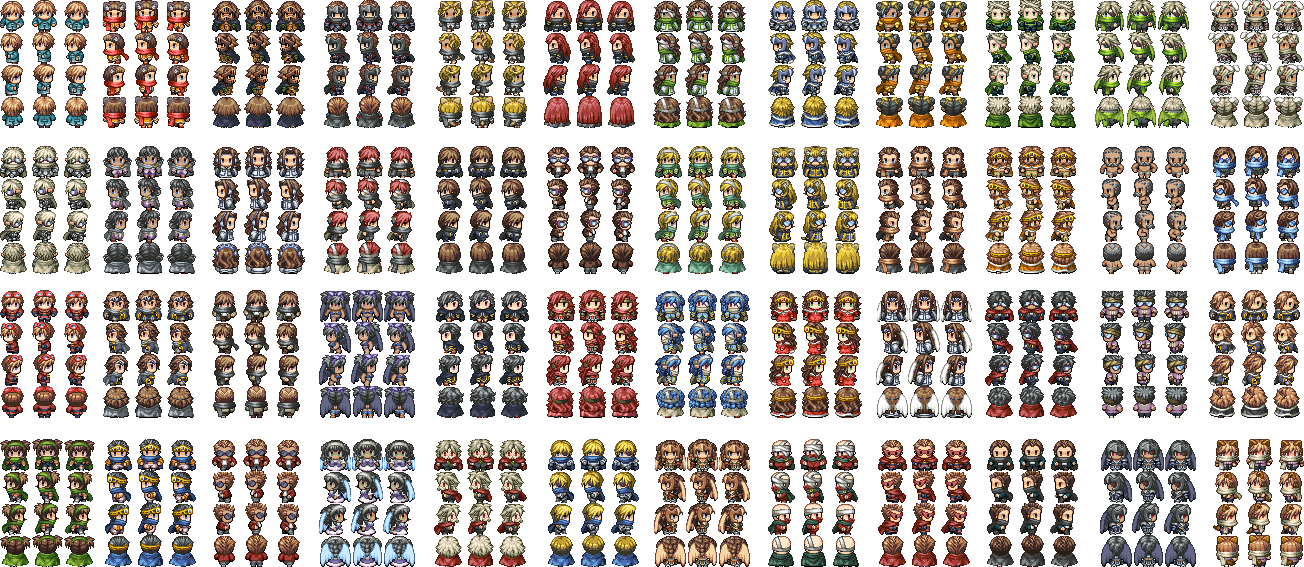
\includegraphics[width=\textwidth]{persos.png}
        \caption{Tileset personnages}
    \end{figure}
    
    \begin{figure}[ht]
        \centering
        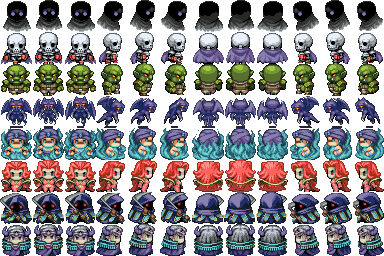
\includegraphics{monsters-32x32.png}
        \caption{Exemple tileset ennemis}
    \end{figure}
    
    \begin{figure}[ht]
        \centering
        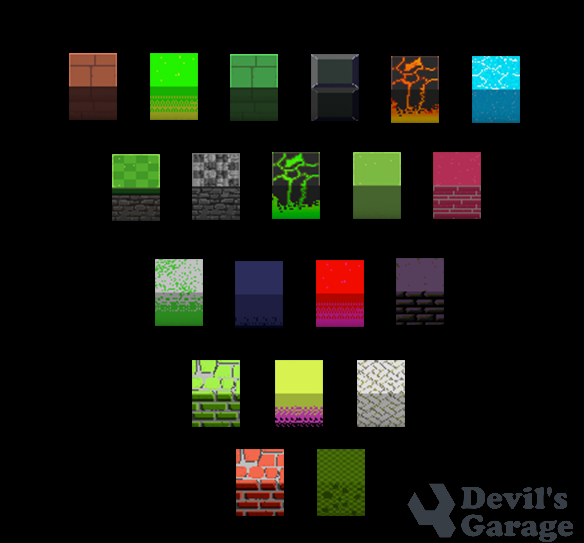
\includegraphics[width=\textwidth]{field.png}
        \caption{Exemple tileset terrain}
    \end{figure}
    
   \begin{figure} [ht]
            \centering
            \begin{subfigure}
                \centering
                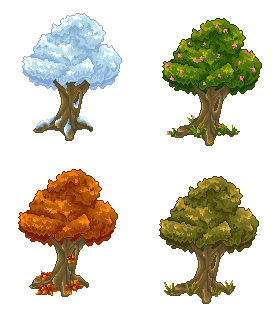
\includegraphics[width=.4\linewidth]{trees.png}
                \caption{Arbres}
            \end{subfigure}%
            \begin{subfigure}
                \centering
                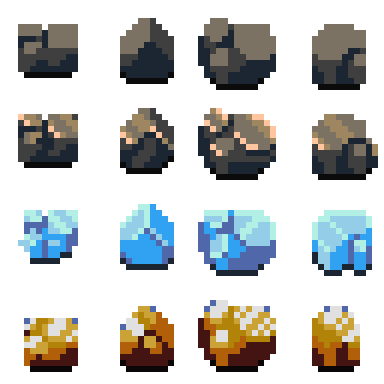
\includegraphics[width=.4\linewidth]{rocks.png}
                \caption{Rochers}
            \end{subfigure}
            \caption{Exemple d'obstacles}
        \end{figure}

\clearpage
\section{Description et conception des états}

\subsection{Description des états}
Un état de jeu est formé de la carte du monde possédant des cases d'un certain élément, repérées par ses coordonnées dans le monde, pouvant éventuellement posséder un obstacle infranchissable inamovible ou un personnage mobile. Ce personnage fait partie d'une équipe possédant un inventaire contenant des objets, ceux-ci étant principalement des armes pouvant être équipées individuellement et possédant diverses capacités et caractéristiques. L'équipe du joueur peut combattre et obtenir des quêtes fournissant des récompenses lors de leur accomplissement.
Le détail des attributs et opérations des différentes classes est présenté ci-dessous.

\subsubsection{State}
\begin{itemize}
\item L'état possède une matrice de pointeurs de cellules qui contiennent toutes les information liées au terrain et à la position des personnages
\item Il possède aussi toutes les équipes de personnages, ainsi que les quêtes et le combat éventuel qui se déroule.
\item L'heure correspondant au nombre de fronts d'horloge, ainsi que la vitesse à laquelle le jeu est actualisé permet d'associer un temps à chaque état du jeu
\item Un booléen indique si l'inventaire est ouvert
\end{itemize}

\subsubsection{Cell}
\begin{itemize}
\item La case doit contenir un élément choisi parmis une énumération et peut contenir un obstacle infranchissable par les personnages
\end{itemize}

\subsubsection{Character}
\begin{itemize}
\item Les coordonnées du personnage et la direction dans laquelle il se tourne
\item Le personnage a un nom et appartient à une race qui sera utile par la suite pour les quêtes notamment
\item Il possède également des attributs utiles au combat lui permettant de se déplacer, d'attaquer et de pouvoir encaisser des attaques
\item Chaque personnage possède enfin une arme lui permettant d'effectuer diverses actions
\end{itemize}

\subsubsection{Team}
\begin{itemize}
\item L'équipe a un nom
\item Elle comprend l'ensemble des personnages aptes au combat. Seul un combattant représente l'équipe hors combat lors du déplacement sur la carte du monde, et seul un nombre limité de personnages peuvent combattre simultanément
\item L'équipe stocke également l'inventaire des objets récupérés, pouvant être affectées aux différents personnages de l'équipe
\end{itemize}

\subsubsection{Inventory}
\begin{itemize}
\item L'inventaire comprend différents objets, entre autres les armes affectées aux combattants et celles en réserve
\end{itemize}

\subsubsection{Weapon}
\begin{itemize}
\item L'arme peut posséder un nom
\item L'arme possède des capacités permettant d'attaquer ou de se défendre
\item Elle possède également un élément de prédilection répercuté sur son porteur
\end{itemize}

\subsubsection{Ability}
\begin{itemize}
\item Les habilités peuvent avoir un nom, coûtent un certain nombre de points d'action, infligent un certain nombre de dégâts (ou de soin en cas de valeur négative) et possèdent éventuellement un temps de recharge de la capacité
\item Elles possèdent un élément répercuté sur l'attaque en elle même. Elle sera souvent du même élément que l'arme, mais pourront parfois différer
\item L'attaque possède une portée effective, et une zone d'effet dépendant du type d'arme utilisé
\item Une réduction de dégât peut être envisagée pour les attaques de zone afin de moins affecter les personnages éloignés du point d'impact
\end{itemize}

\subsubsection{Fight}
\begin{itemize}
\item Le combat enregistre le nombre de tours passés afin de définir la prochaine équipe à jouer
\item Il possède les différentes équipes se battant afin que chaque membre de l'équipe puisse se déployer avant de commencer
\end{itemize}

\subsubsection{MainQuest}
\begin{itemize}
\item Les quêtes principales s'obtiennent avant d'entrer en phase de combat en effectuant certaines actions et peuvent se décliner en divers objectifs à remplir à travers plusieurs combats à travers ses classes filles
\end{itemize}


\subsection{Conception Logiciel}
Le diagramme des classes pour les états est présenté en Figure 8 : 
\begin{itemize}
\item La classe en vert contient les information globales sur le déroulement du jeu et permettent de déterminer l'état actuel du jeu
\item Les classes en jaune caractérisent les personnages et le terrain dans lequel ils évoluent
\item Les classes en bleu déterminent les actions possibles par les différents personnages
\item Les classes en rouge permettent d'implémenter les phases de combat ainsi que les quêtes, permettant d'obtenir du matériel ou de nouveaux membres d'équipe.
\end{itemize}

\begin{landscape}
    \begin{figure}[p]
    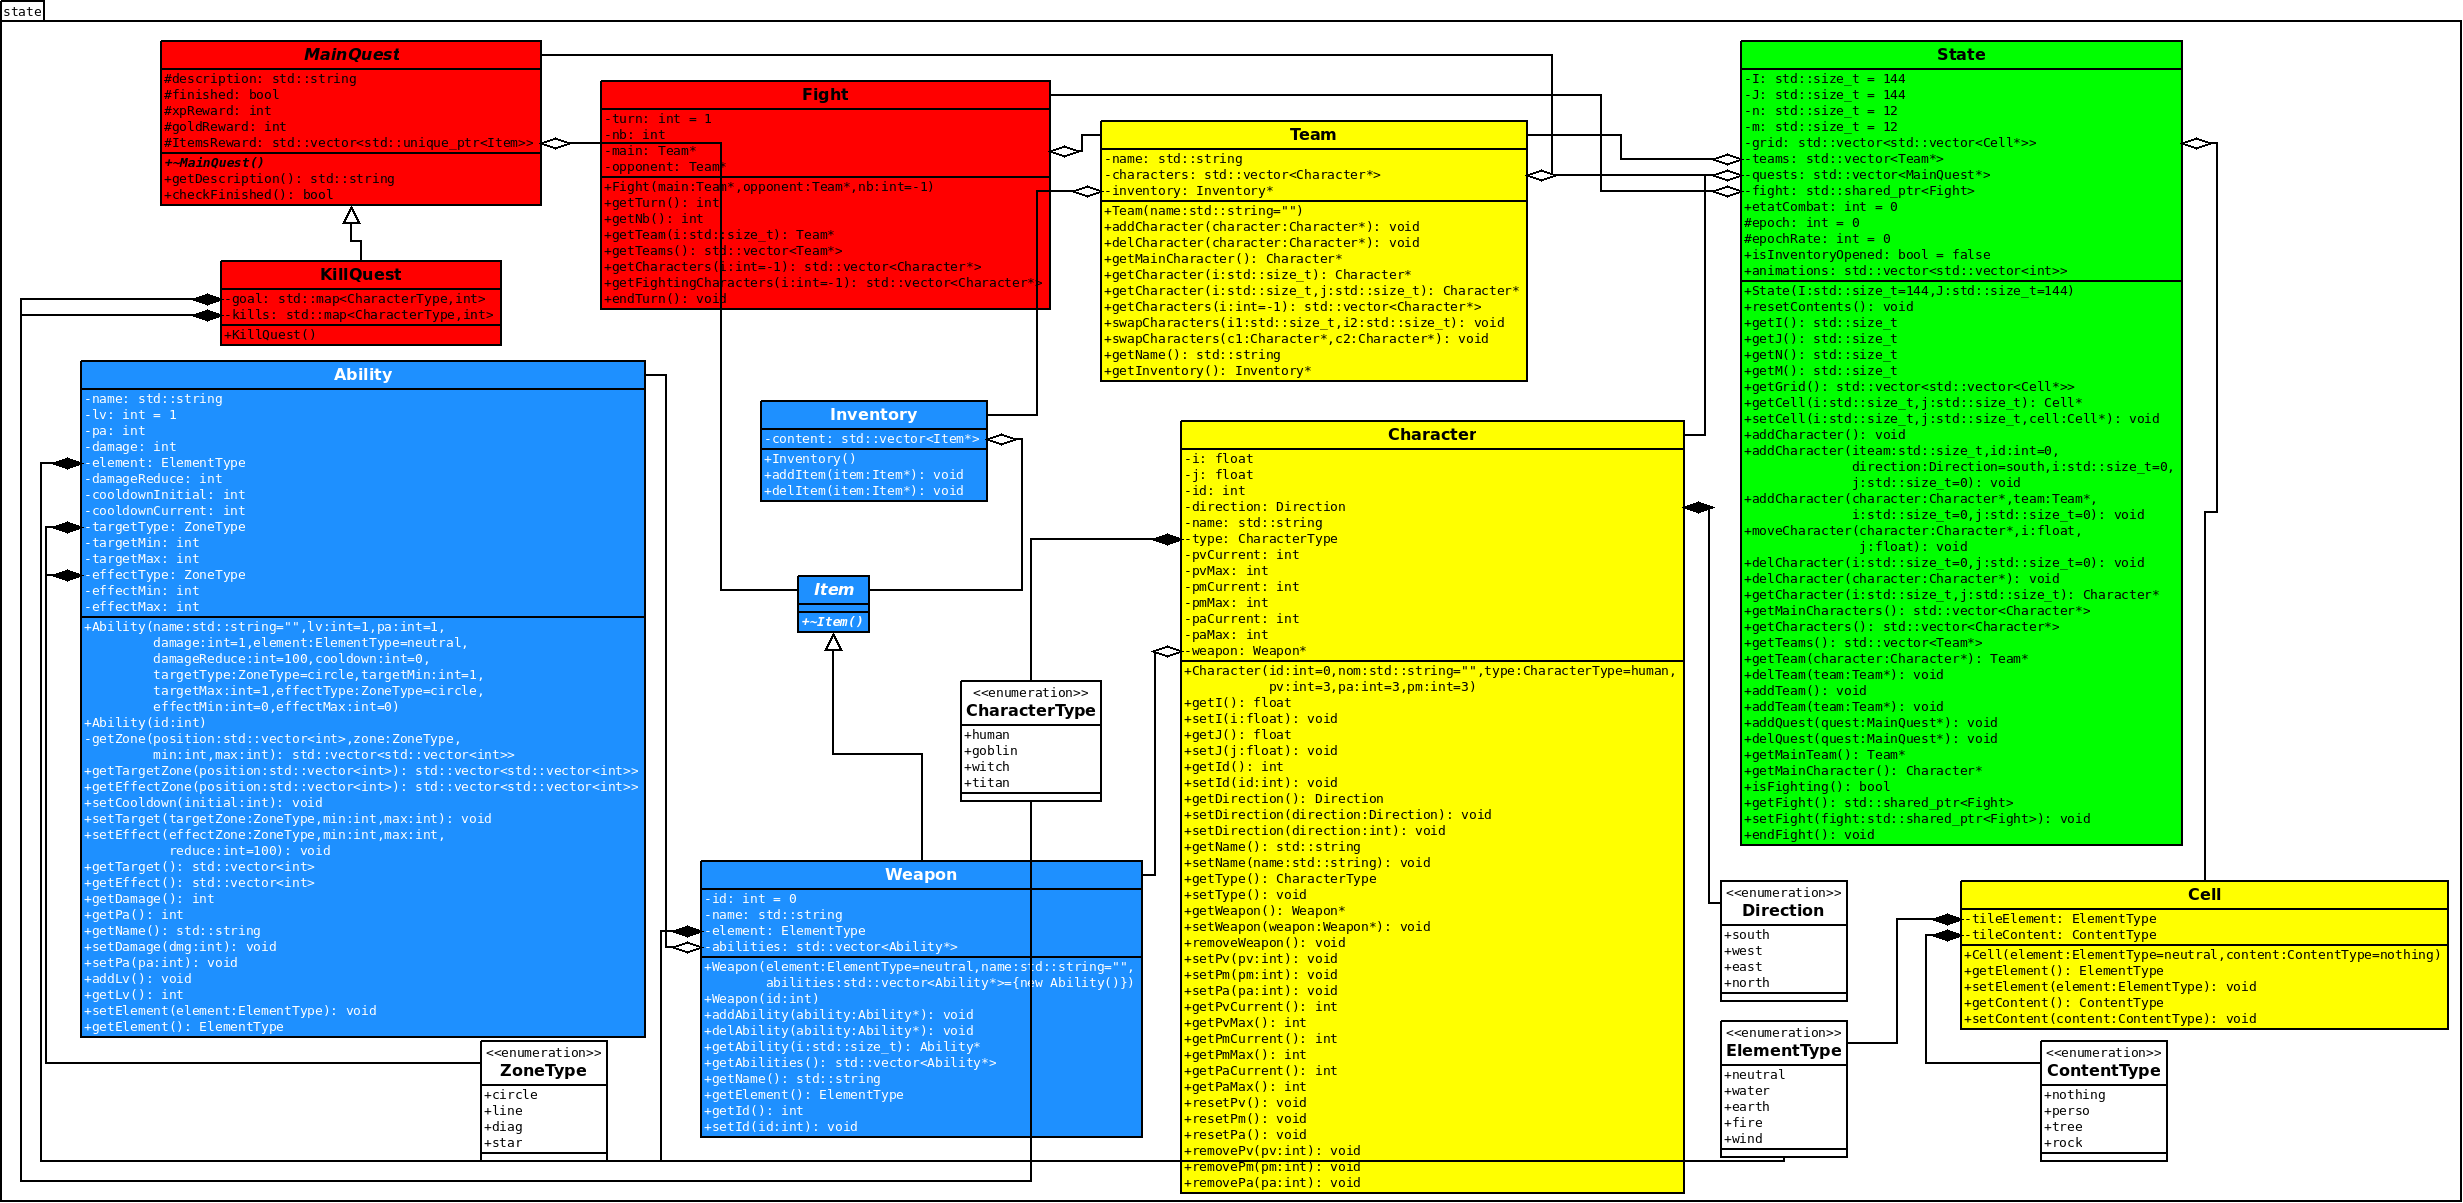
\includegraphics[width=0.9\paperheight]{state.png}
        \caption{\label{uml:render}Diagramme des classes de rendu.} 
    \end{figure}
\end{landscape}

\clearpage
\section{Rendu : Stratégie et Conception}

\subsection{Stratégie de rendu d’un état}
Le rendu de l'état est possible grâce aux différentes informations récupérées de la classe World, c'est à dire les tuiles et les personnages. Il s'agit donc d'un rendu à 3 couches successives. Toutes les textures sont chargées et découpées afin de renvoyer le sprite correspondant à un personnage donné ou à une cellule du monde donnée (élément et contenu optionnel). Ce sprite est ensuite déplacé au lieu d'en générer un nouveau. Un système de vue centre la fenêtre sur une petite zone autour du personnage principal (encadré d'un carré blanc) et n'actualise l'affichage des sprites sur cette vue uniquement et pas sur le monde entier. Cela évite d'une part de charger des sprites inutilement et d'autre part de créer une carte du monde où les zones pas encore visitées ne seraient pas visibles (ce serait alors une vue du monde en entier).


\subsection{Conception logiciel}

 Le diagramme de classes du rendu est présenté en Figure 9 : 
\begin{itemize}
\item Les classes en vert sont les gestionnaires des différentes ressources. Elles chargent les différentes textures du jeu lors de l'instanciation en prenant en argument leur résolution et possèdent la méthode getSprite() générant le sprite redimensionné aux dimensions des cellules, compatible avec l'état du monde, dépendant alors de la tuile à afficher (élément + contenu) et du personnage à afficher.
\item Render réutilise alors les sprites générés pour afficher la carte grâce au RenderWindow de sfml et gère la View correspondante via display().
\end{itemize}

Une partie des classes n'a pas pu être représentée sur le dia vu que ces classes présentent des méthodes constantes et que dia ne gère pas ce type de fonctions. En conséquence ces headers ont été rédigés à la main. Les classes qui n'ont pas pu être incluses sont les suivantes:
\begin{itemize}
    \item IGWindow\\
    La classe permet d'afficher une fenêtre qu'on peut déplacer et fermer par dessus la vue du monde
    \item IGWindowContainer\\
    Comme son nom l'indique celle classe contient l'ensemble des fenêtres, lorsque on souhaite ajouter une fenêtre à la vue de notre jeu il faut l'enregistrer auprès du gestionnaire de window. Le gestionnaire s'occupe du déplacement et de la fermeture des fenêtres qu'il contrôle.
    \item UIInventory\\
    La classe permet d'afficher l'inventaire d'une team. La classe hérite de IGWindow, il est donc possible de déplacer et fermer la fenêtre.
\end{itemize}

\begin{figure}[ht]
    \centering
    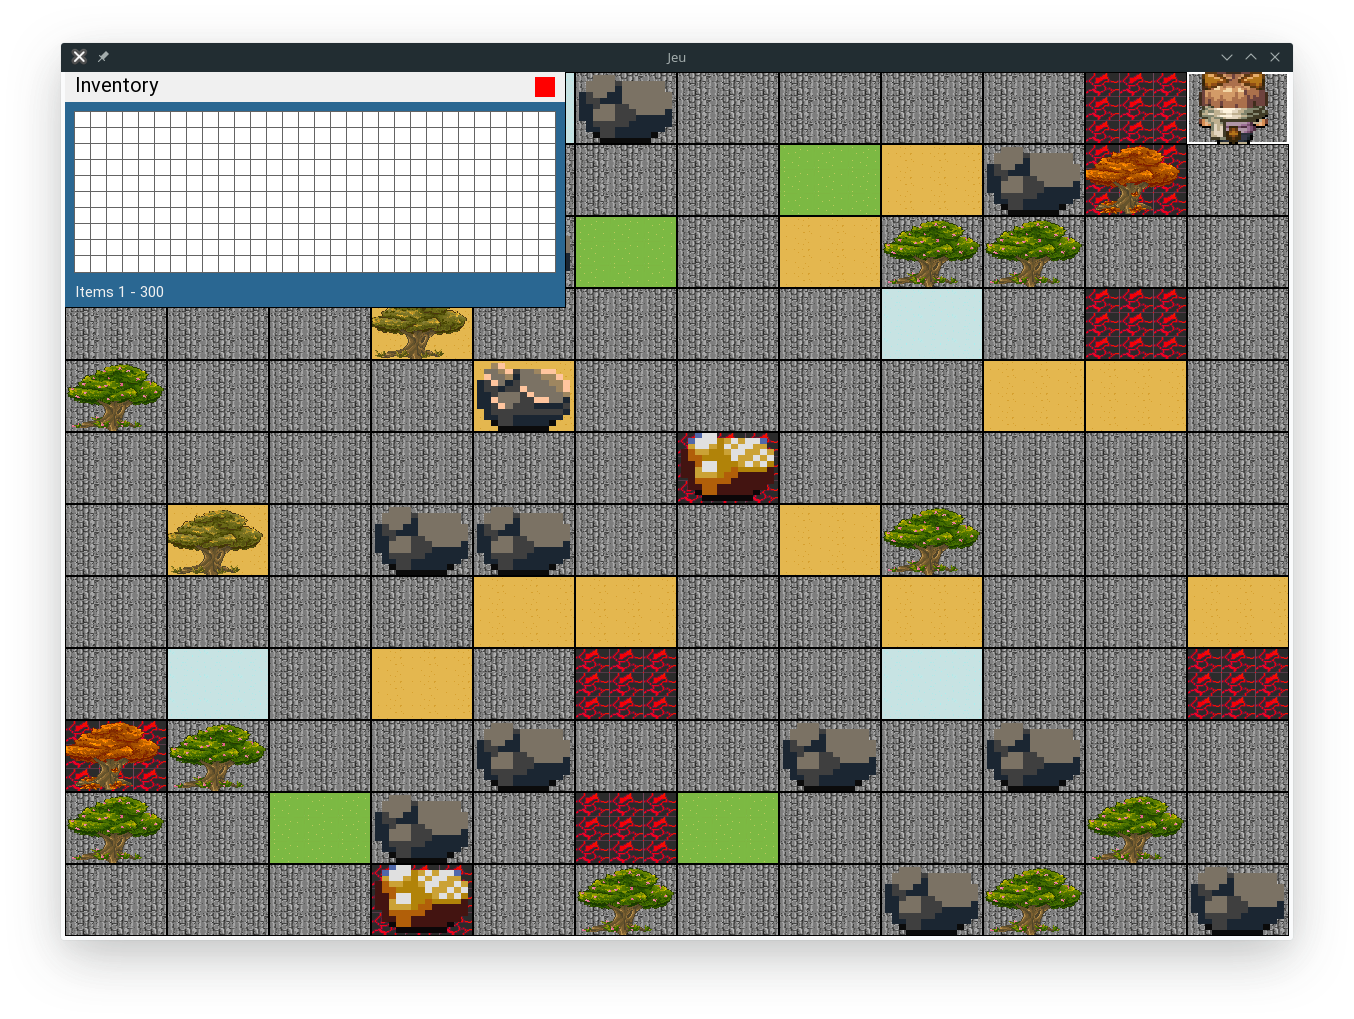
\includegraphics[width=\textwidth]{render_preview.png}
    \caption{Preview du rendu}
\end{figure}

\begin{landscape}
    \begin{figure}[p]
        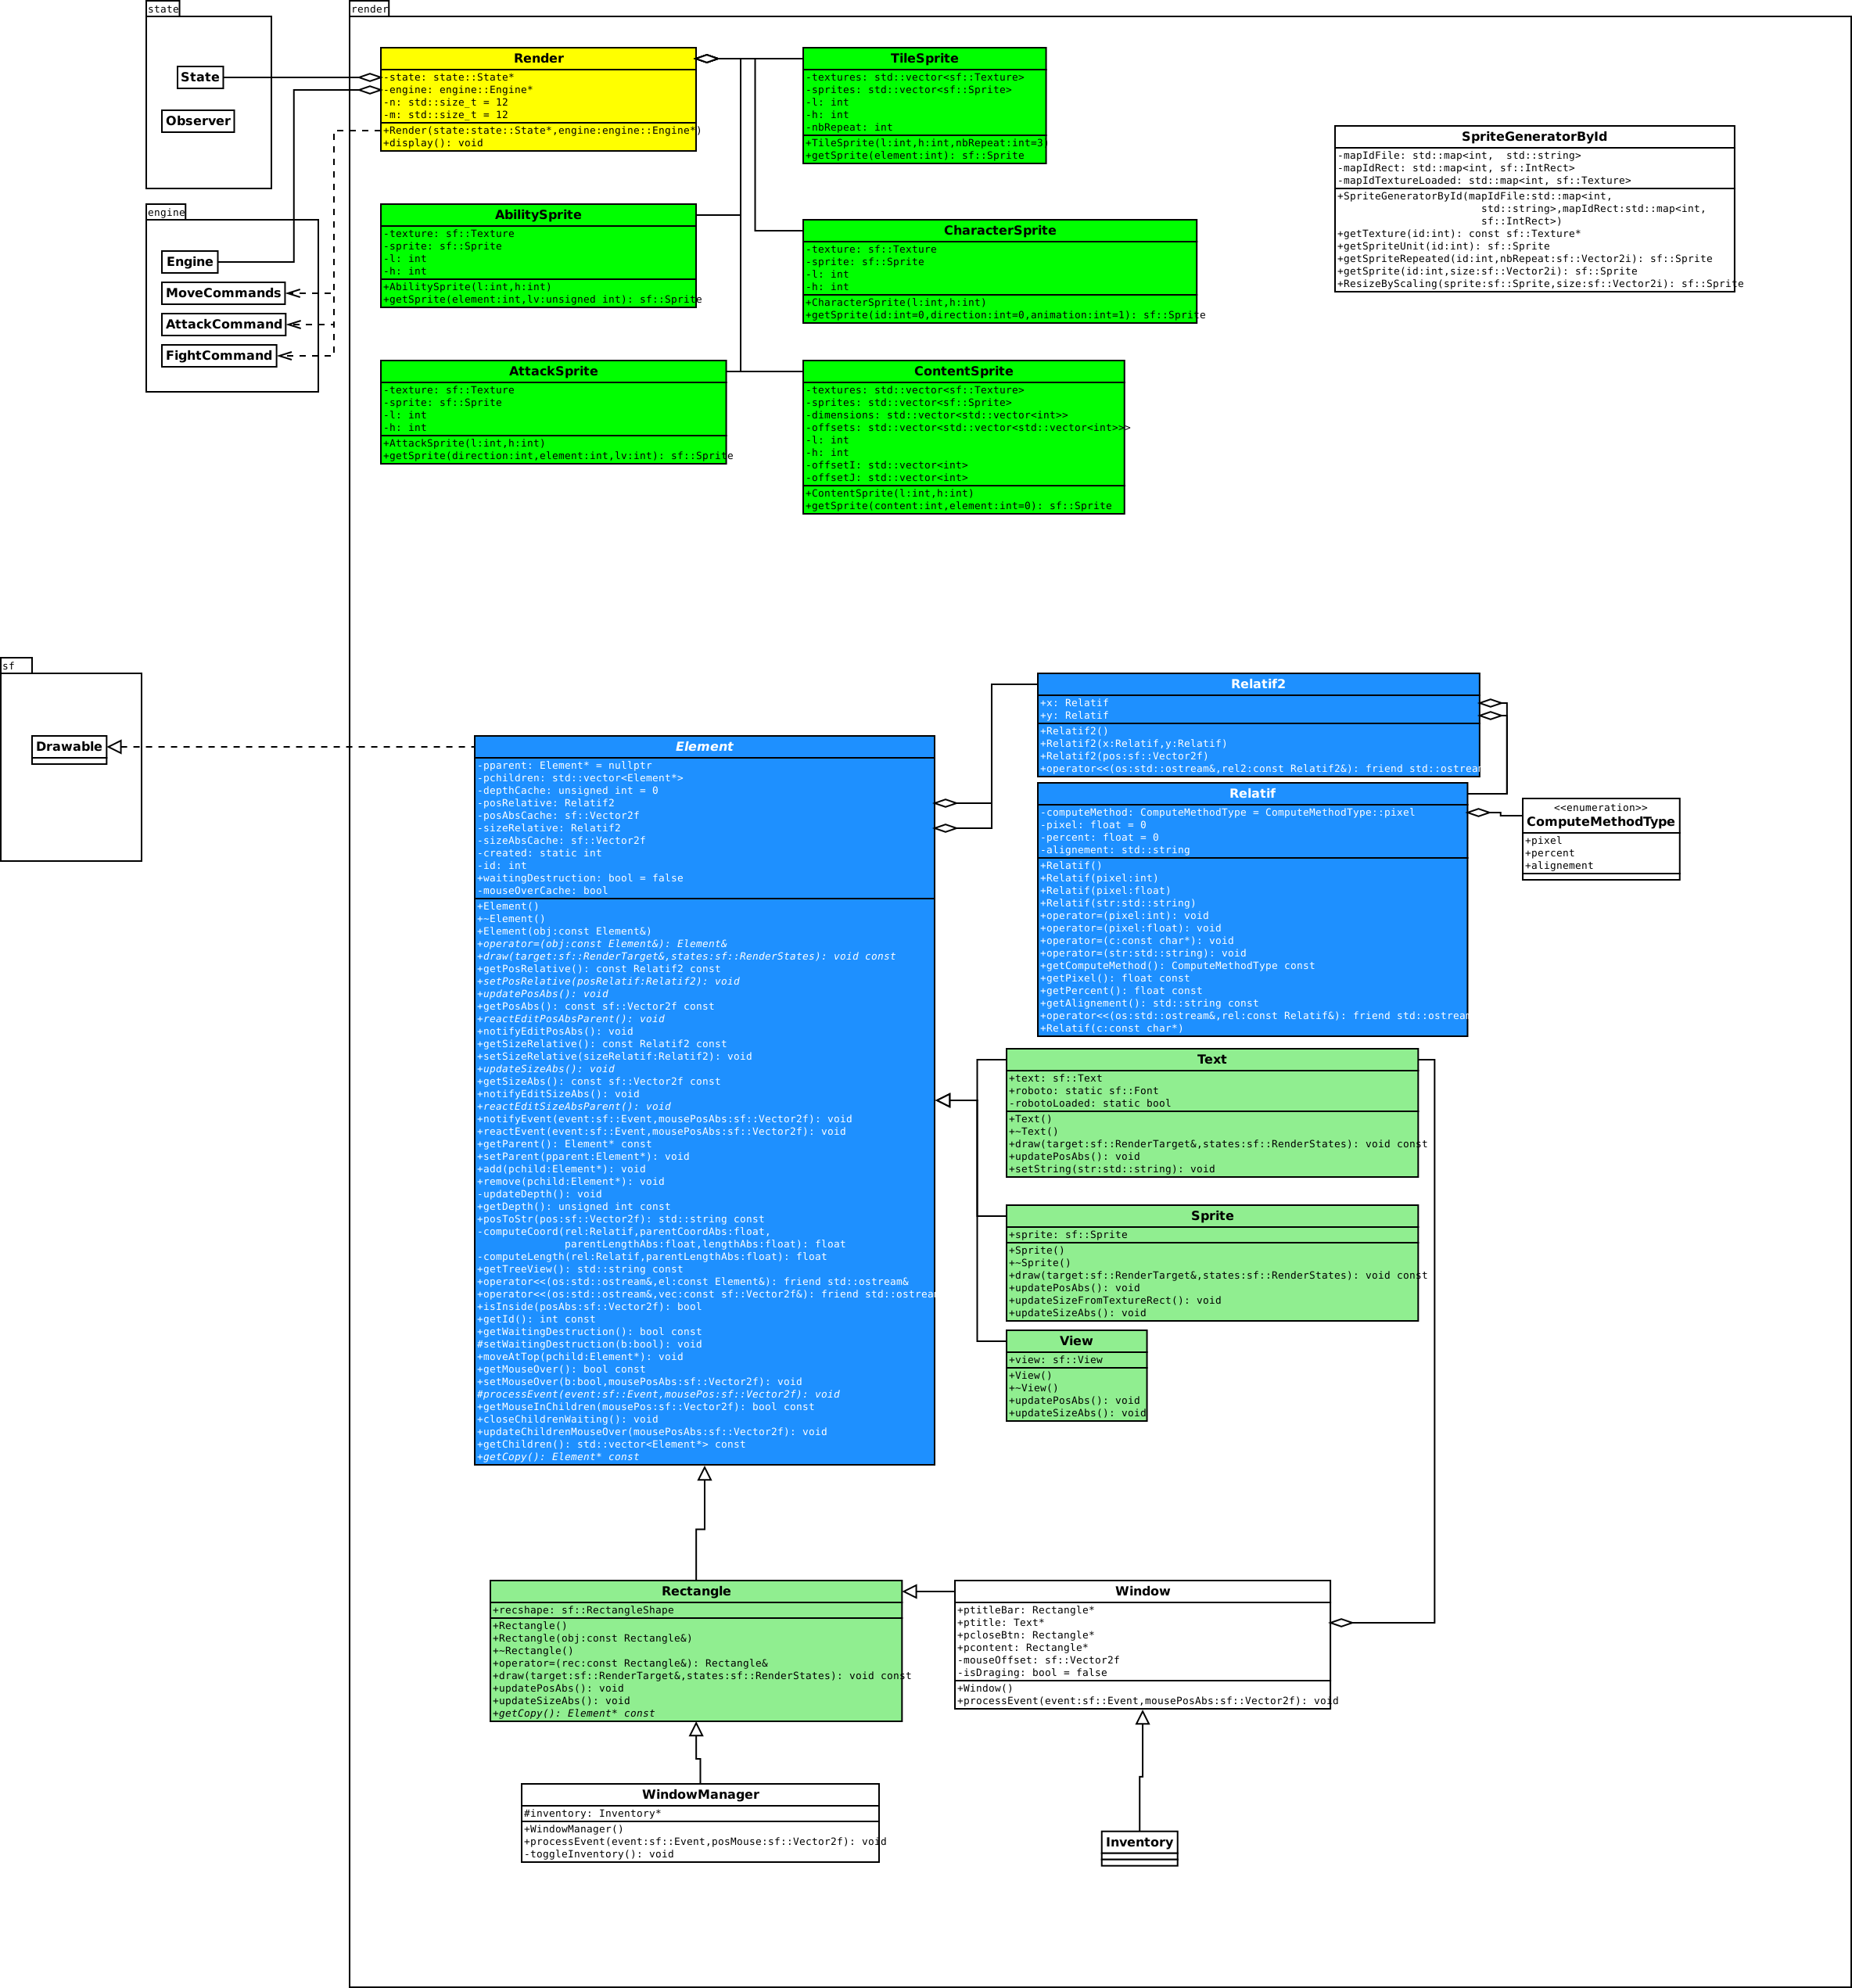
\includegraphics[width=0.9\paperheight]{render.png}
        \caption{\label{uml:engine}Diagramme des classes de rendu.}
    \end{figure}
\end{landscape}

\section{Règles de changement d'états et moteur de jeu}

\subsection{Horloge globale}
	Les commandes sont exécutées à une fréquence de 30 Hz et chaque animation de déplacement est constitué d'une étape de changement de direction ainsi que de 12 étapes de déplacement pur séparés en 4 sprites différents.


\subsection{Changements extérieurs}
	Les changements extérieurs sont le déplacement du personnage, que ce soit en combat ou non, ainsi que les phases d'attaque en combat.


\subsection{Changements autonomes}
	Les changements autonomes sont le changement de direction du personnage lors de son déplacement, ainsi que le démarrage de la phase de combat permettant de déployer tous les personnages de chaque équipe si un ennemi est rencontré lors de la phase d'exploration.

\subsection{Conception logiciel}

Le diagramme des classes pour le moteur du jeu est présenté en Figure 11. Le moteur de jeu repose sur le pattern Command et permet la mise en oeuvre différée des commandes modifiant l'état du jeu.

\textbf{Classes Command} Ces classes représentent les commandes exécutées par le moteur. 
\begin{itemize}
\item MoveCommands permet de générer l'ensemble des commandes individuelles MoveCommand et DirectionCommand afin de créer une animation de déplacement en utilisant un pathfinding A* (rapide mais ne générant pas nécessairement le chemin le plus optimal) et FightCommant en cas de rencontre avec un ennemi, ce qui lance la phase de combat.
\item AttackCommand permet aux différents personnages d'attaquer avec leurs capacités et ainsi d'infliger des dégâts à différentes cibles.
\end{itemize}


\textbf{Engine} Le moteur exécute les commandes dans l'ordre d'apparition


\begin{landscape}
    \begin{figure}[p]
        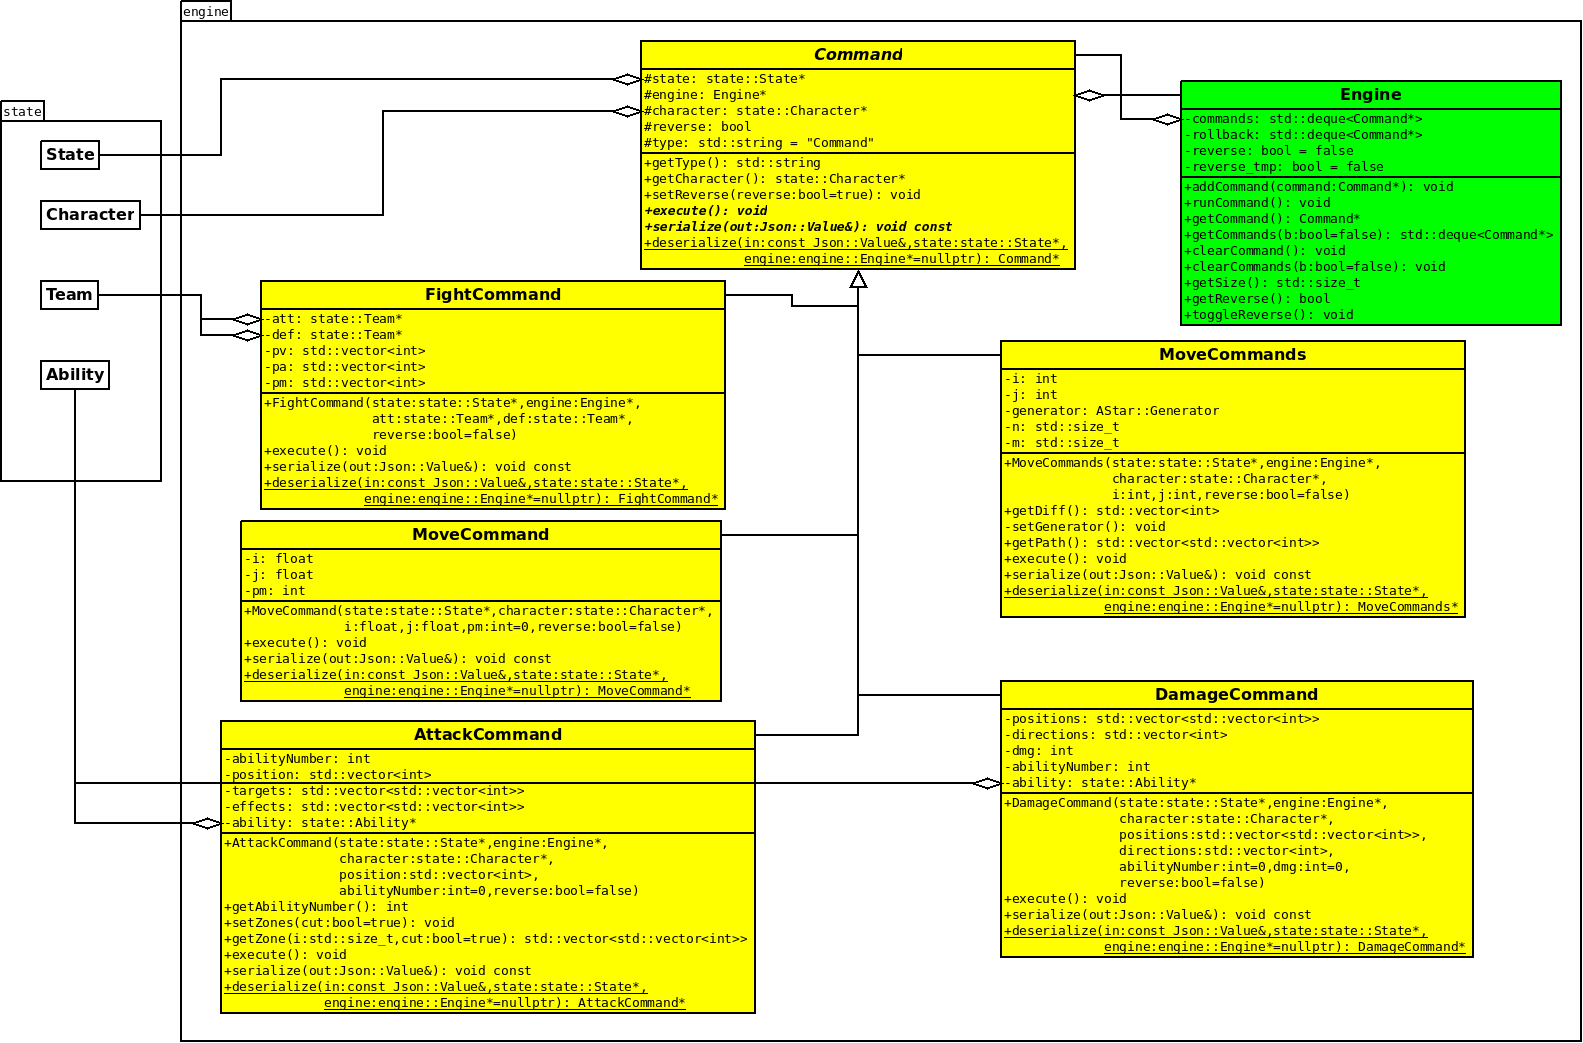
\includegraphics[width=0.9\paperheight]{engine.png}
        \caption{\label{uml:engine}Diagramme des classes du moteur.}
    \end{figure}
\end{landscape}

\clearpage
\section{Intelligence Artificielle}

\subsection{Stratégies}

\clearpage
\subsection{Conception logiciel}


%\begin{landscape}
%\begin{figure}[p]
%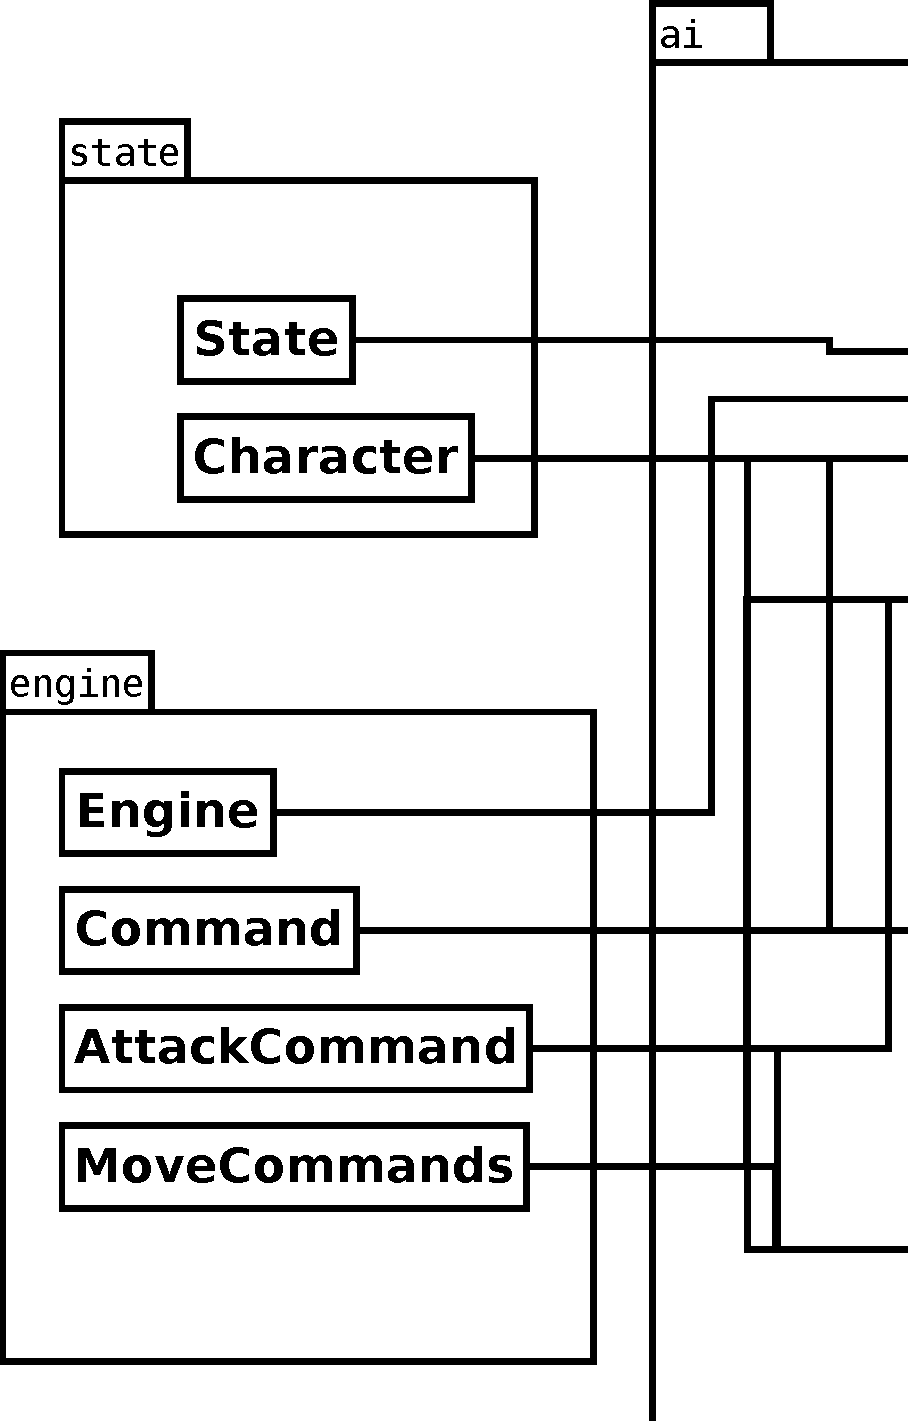
\includegraphics[width=0.9\paperheight]{ai.pdf}
%\caption{\label{uml:ai}Diagramme des classes d'intelligence artificielle.} 
%\end{figure}
%\end{landscape}


\section{Modularisation}
\label{sec:module}

\subsection{Organisation des modules}

\clearpage
\subsection{Conception logiciel}


%
%\begin{landscape}
%\begin{figure}[p]
%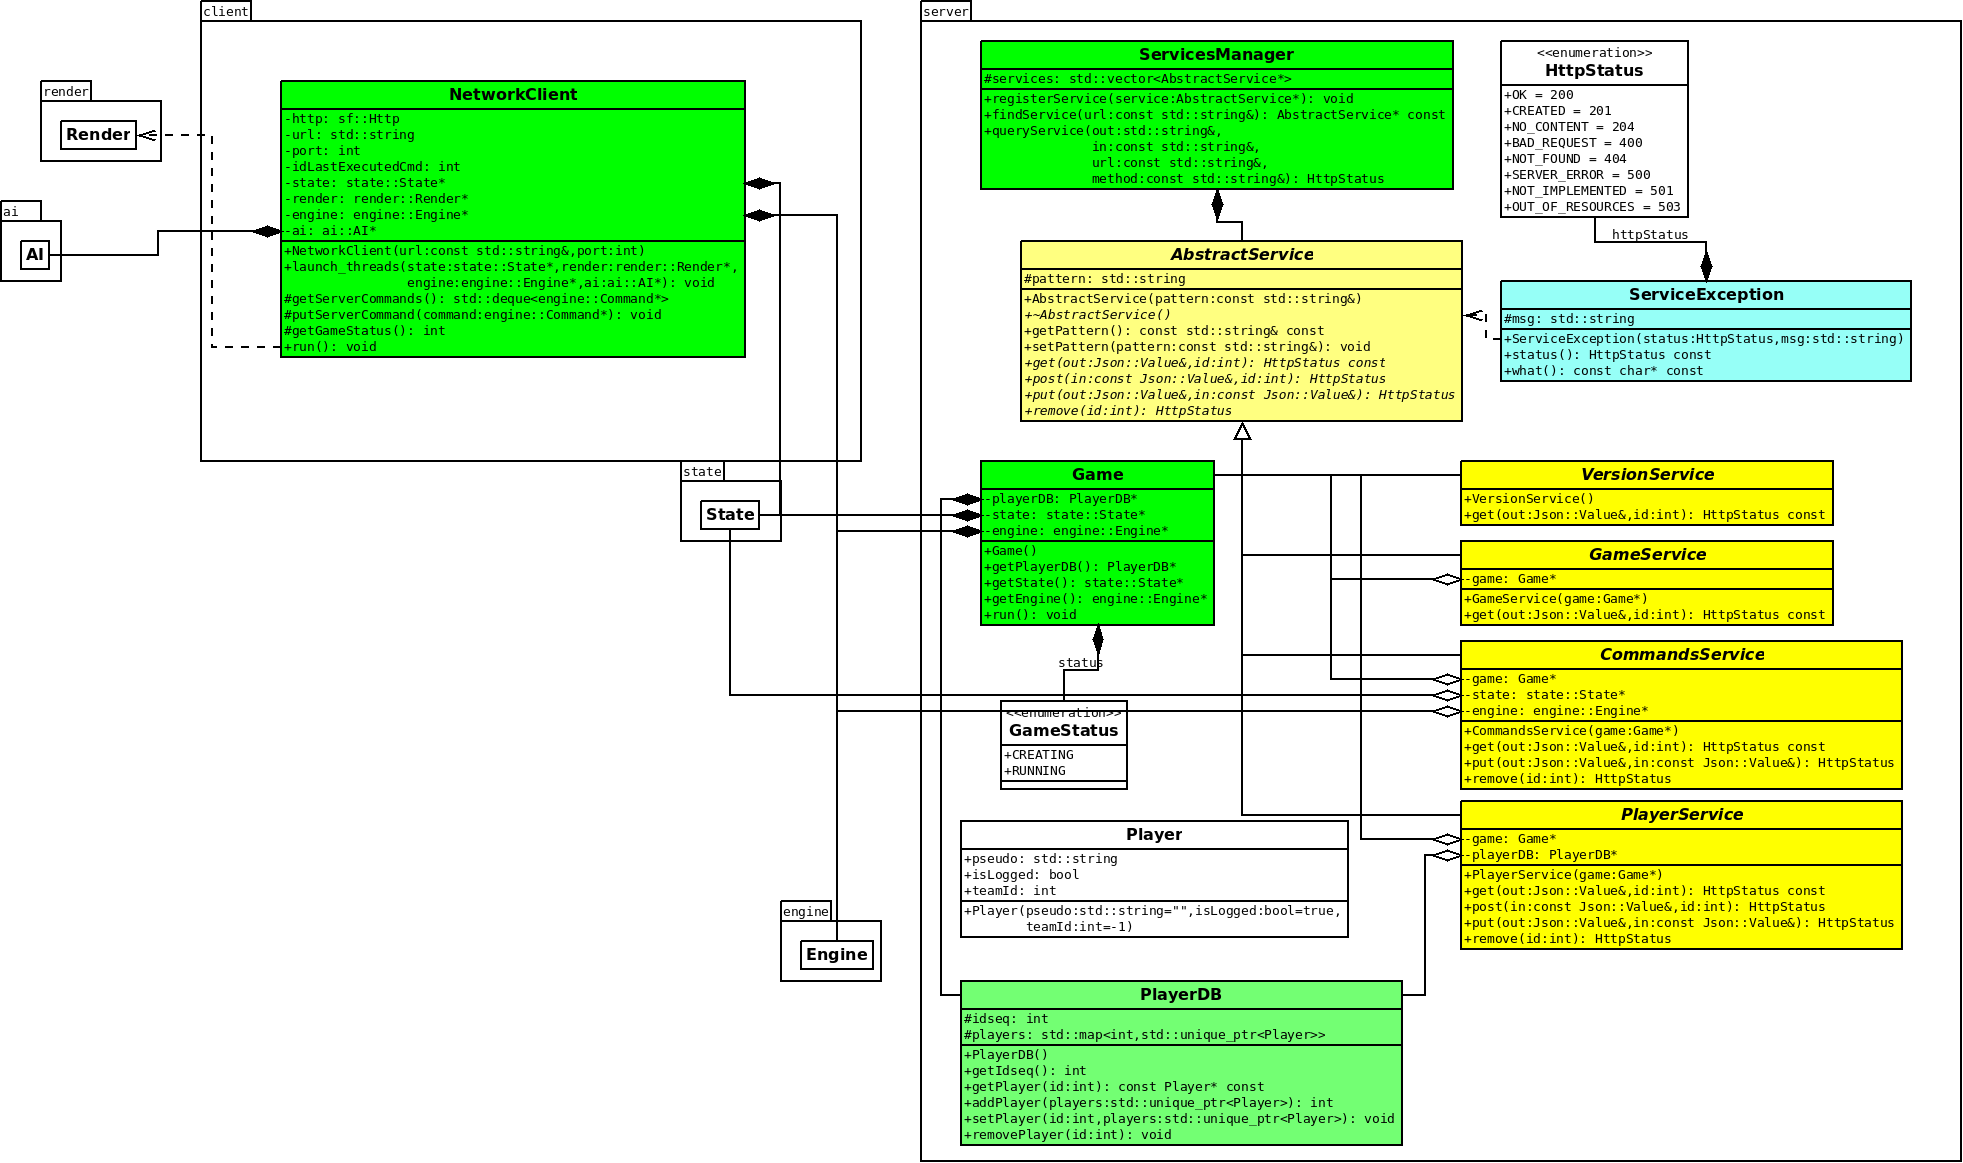
\includegraphics[width=0.9\paperheight]{module.pdf}
%\caption{\label{uml:module}Diagramme des classes pour la modularisation.} 
%\end{figure}
%\end{landscape}

\end{document}

